\section{SIMETRÍAS CONTINUAS Y GRUPOS DE LIE}
$\bullet$ \textbf{Transformaciones:} Descritas por parámetros continuos (ej. ángulos).\\ Invariancia de $H$ bajo transf. $\Leftrightarrow U(\theta) HU(\theta)^{-1} = H$  $\implies$ leyes de conservación.\\
$\bullet$ \textbf{Generadores ($J$):} Operadores hermíticos que construyen la transformación finita.
$$ U(\theta) = e^{i \sum_a \theta_a J_a} $$
$\bullet$ \textbf{Parámetros ($\theta$):} Parámetros de la transformación, $\theta \in \mathbb{R}$, continuos.\\
$\bullet$ \textbf{Conmutación:} $[H, J_a] = 0 \implies$ Generadores son constantes de movimiento.\\

$\bullet$  \textbf{Invariancia del subespacio:} $\text{Dado } \{|n\rangle\} \text{ tal que } H|n\rangle = E_n|n\rangle \quad \text{y} \quad [H, J_a] = 0:$ \\
$H(J_a|n\rangle) = J_a H |n\rangle = E_n (J_a|n\rangle) \implies J_a|n\rangle \text{ autoestado de } H \text{ con mismo autovalor } E_n.$

$\bullet$ \textbf{Degeneración:} Si $[H, J_a] = 0$ y $[J_a, J_b] \neq 0$, los autoestados de $H$ forman multipletes degenerados (misma energía $E_n$).

\section{GRUPO DE ROTACIONES SO(3)}
$\bullet$ \textbf{Definición:} Matrices $3\times3$ ortogonales ($O^TO=I$) con $\det O = +1$.\\
$\bullet$ \textbf{Generadores:} 3 operadores de momento angular $J_1, J_2, J_3$.\\
$\bullet$ \textbf{Álgebra de Lie SO(3):} $ [J_a, J_b] = i \epsilon_{abc} J_c $\\
$\bullet$ \textbf{Operadores Escalera:}
$$ J_\pm = J_1 \pm i J_2 \quad \qquad J_\pm |j,m\rangle = \sqrt{(j \mp m)(j \pm m + 1)} |j, m \pm 1\rangle $$\vspace{-2pt}
$$J_3 |j,m\rangle = m | j,m\rangle \qquad J^2|j,m\rangle = j(j+1)|j,m\rangle$$
$\bullet$ \textbf{Producto Tensorial (Adición de Momento Angular):}\\
Composición de dos partículas de espín/isospín $j_1$ y $j_2$.
$$|j_1, m_1\rangle \otimes |j_2, m_2\rangle = |J,M\rangle \quad {J} = j_1 + j_2: |j_1-j_2| \le J \le j_1+j_2 \quad M = m_1+m_2\quad |M|\leq J$$
\textbf{Clebsch-Gordan Coefficients:} $|J,M\rangle = \sum_{m_1,m_2} \langle j_1 m_1 j_2 m_2 | J M \rangle |j_1 m_1\rangle |j_2 m_2\rangle$.\\
$\bullet$ \textbf{Representaciones Irreducibles (Irreps):} \\
- Caracterizadas por momento angular $j$ (entero o semientero). \\ 
- Dimensión: $d = 2j+1$.\\
- Base: $\{|j,m\rangle\}$ con $m \in \{-j, -j+1, \dots, j-1, j\}$.\\
$\bullet$ \textbf{Casimir:} $J^2 = \sum J_a^2$ conmuta con todos los $J_a$.

\section{GRUPOS SU(n) - SIMETRÍAS INTERNAS}
$\bullet$ \textbf{Definición:} Matrices $n\times n$ unitarias ($U^\dagger U = I$) con $\det U = 1$. ``Special Unitary".\\
$\bullet$ \textbf{Generadores:}  Hermíticos ($T_a^\dagger = T_a$) y Traza nula ($\text{Tr}(T_a)=0$).\\
- Número de generadores independientes: $N=n^2 - 1$.\\
$\bullet$ \textbf{Rango:} Número de generadores diagonales simultáneamente diagonalizables = $n-1$.

\section{GRUPO SU(2) - ISOSPÍN}
$\bullet$ \textbf{Generadores:} $N = 2^2 - 1 = 3$. Relación con matrices de Pauli $\sigma_a$: $ T_a = \frac{\sigma_a}{2}$\\
$\bullet$ \textbf{Álgebra SU(2):} $[T_a, T_b] = i \epsilon_{abc} T_c$ (Isomorfa a SO(3)).\\
$\bullet$ \textbf{Irreps Fundamentales:} Autoestados comunes a $T^2, T_3.$ $T_3$ único generador diagonal.\\
1. \textbf{Doblete ($\mathbf{2}$):} $j=1/2$. Dim=2. Rep. fundamental.
   Base: $|\frac{1}{2}, \frac{1}{2}\rangle = \binom{1}{0}, |\frac{1}{2}, -\frac{1}{2}\rangle = \binom{0}{1}$.\\
2. \textbf{Triplete ($\mathbf{3}$):} $j=1$. Dim=3. Rep. adjunta.
   Base: $|1,1\rangle, |1,0\rangle, |1,-1\rangle$.\\
3. \textbf{Singlete ($\mathbf{1}$):} $j=0$. Dim=1. Invariante escalar. Base: $|0, 0\rangle$\\
4. \textbf{Cuadruplete ($\mathbf{4}$):} $j=3/2$ Dim=4. .\\
- Cada estado $|j,m\rangle$ se transforma en los otros bajo la acción de $T_{\pm}$:\\
\noindent
\begin{minipage}{\linewidth}
\centering
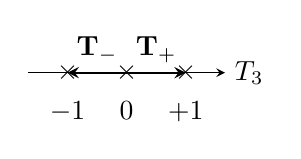
\begin{tikzpicture}[scale=0.5, >=stealth]
    % --- CONFIGURACIÓN ---
    % Eje de coordenadas (Solo existe T3)
    \draw[->, thin] (-2.5,0) -- (2.5,0) node[right] {$T_3$};

    % Coordenadas de las raíces (Valores propios del operador adjunto)
    \coordinate (O) at (0,0);
    \coordinate (Tp) at (1.5, 0);   % T+ (Sube isospín)
    \coordinate (Tm) at (-1.5, 0);  % T- (Baja isospín)

    % --- VECTORES (RAÍCES) ---
    % Mismo estilo: ultra thick
    \draw[->, thick] (O) -- (Tp) node[midway, above] {$\textbf{T}_+$};
    \draw[->,  thick] (O) -- (Tm) node[midway, above] {$\textbf{T}_-$};

    % --- CRUCES EN LOS VÉRTICES ---
    \node at (Tp) [label=below:{ $+1$}] {$\times$};
    \node at (Tm) [label=below:{ $-1$}] {$\times$};
    \node at (O)  [label=below:{ $0$}]  {$\times$}; % El centro (Cartan)

\end{tikzpicture}
\end{minipage}
- Los representantes de los generadores de SU(2) son matrices $(2j+1)\times (2j+1)$.\\
- A partir de dos multipletes $A, B$ con $j_A, j_B$ tal que $A= 2j_A+1, B=2j_B+1$,
se pueden descomponer, empleando coeficientes de C.G., en otros multipletes tal que: $$\mathbf{A} \otimes \mathbf{B} = \bigoplus_{J=|j_A - j_B|}^{j_A + j_B} \mathbf{(2J+1)} \;\;\; \rightarrow \;\;\; \prod \dim_{\otimes} = \sum \dim_{\oplus} \quad \text{e.g.}
\begin{array}{cc}
     \textbf{2} \otimes \textbf{2} = \textbf{3}\oplus \textbf{1}  \\
     \textbf{2}\otimes \textbf{3} = \textbf{4} \oplus \textbf{2}
\end{array}$$\\


\hypertarget{su3}{\section{GRUPO SU(3) - MODELO DE QUARKS}}
$\bullet$ \textbf{Generadores:} $N = 3^2 - 1 = 8$. Relación con matrices de Gell-Mann $\lambda_a$: $F_a = \frac{\lambda_a}{2}$.\\
\begin{align*}
&\lambda_1 = \left(\begin{smallmatrix}0&1&0\\1&0&0\\0&0&0\end{smallmatrix}\right)&\lambda_2 = \left(\begin{smallmatrix}0&-i&0\\i&0&0\\0&0&0\end{smallmatrix}\right)&\qquad\lambda_3 = \left(\begin{smallmatrix}1&0&0\\0&-1&0\\0&0&0\end{smallmatrix}\right)&\lambda_4 = \left(\begin{smallmatrix}0&0&1\\0&0&0\\1&0&0\end{smallmatrix}\right)\\
&\lambda_5 = \left(\begin{smallmatrix}0&0&-i\\0&0&0\\i&0&0\end{smallmatrix}\right)&\lambda_6 = \left(\begin{smallmatrix}0&0&0\\0&0&1\\0&1&0\end{smallmatrix}\right)&\qquad \lambda_7 = \left(\begin{smallmatrix}0&0&0\\0&0&-i\\0&i&0\end{smallmatrix}\right)&\lambda_8 = \frac{1}{\sqrt{3}}\left(\begin{smallmatrix}1&0&0\\0&1&0\\0&0&-2\end{smallmatrix}\right)
\end{align*}


$\bullet$ \textbf{Álgebra SU(3):} $ [F_a, F_b] = i f_{abc} F_c$ \quad $f_{abc}$: Ctes de estructura totalmente antisim.\\
$f_{123}=1$, $f_{147} = f_{246} = f_{257} = f_{345} = \frac{1}{2}$, $f_{156} = f_{367} = -\frac{1}{2}$, $f_{458} = f_{678} = \frac{\sqrt{3}}{2}$.\\
- Asimetría: $f_{abc} = -f_{bac} = -f_{cba} = -f_{acb}$\;\;\; $f_{abc} = f_{bca} = f_{cab}$ \;\;\; resto: nulos.\\

$\bullet$ \textbf{Subálgebra de Cartan (Rango 2):}
Los generadores diagonales conmutan $[F_3, F_8]=0$.
1. Isospín ($T_3$): $T_3=F_3 = \frac{1}{2}\text{diag}(1, -1, 0)$.\\
2. Hipercarga ($Y$): $Y = \frac{2}{\sqrt{3}}F_8 = \text{diag}(\frac{1}{3}, \frac{1}{3}, -\frac{2}{3})$.\\
Los autoestados se etiquetan por $(t_3, y)$ en un plano 2D.\\
$\bullet$ \textbf{Relación de Gell-Mann-Nishijima}:
$ Q = T_3 + \frac{Y}{2} \quad \text{con} \quad T_3 = I_3, \quad Y = B + S $.\\
$Q\equiv$ carga eléctrica (generador de SU(1)$_{\text{EM}}$), $B\equiv$ número bariónico, $S\equiv$ extrañeza
\begin{center}
\begin{tabular}{|c|c|c|c|c|c|c|}
\hline
\hyperlink{quarks_table}{\textbf{q}} & \textbf{$Q$} & \textbf{$T_3$} & \textbf{$Y$} & \textbf{$S$} & \textbf{$B$} & \textbf{spin}\\ \hline
$u$ & $+2/3$ & $+1/2$ & $+1/3$ & $0$ & $1/3$ & $1/2$ \\ \hline
$d$ & $-1/3$ & $-1/2$ & $+1/3$ & $0$ & $1/3$&$1/2$\\ \hline
$s$ & $-1/3$ & $0$ & $-2/3$ & $-1$ & $1/3$ & $1/2$\\ \hline
\end{tabular}\\[2pt]
Antiquarks: todos los números $Q,T_3, Y, S,B$ opuestos.
\end{center}
$\bullet$ \textbf{Operadores Escalera (Raíces):}
Se definen 3 tipos de espín en el plano $(T_3, Y)$:\\

\noindent
% BLOQUE TEXTO (55% del ancho de la columna)
\begin{minipage}[c]{0.58\linewidth}
    \raggedright % Evita espacios feos en líneas cortas
1. \textbf{I-spin ($T_\pm$):} $F_1 \pm iF_2$. $\Delta T_3 = \pm 1, \Delta Y = 0$.\\
2. \textbf{V-spin ($V_\pm$):} $F_4 \pm iF_5$. $\Delta T_3 = \mp 1/2, \Delta Y = \pm 1$.\\
3. \textbf{U-spin ($U_\pm$):} $F_6 \pm iF_7$. $\Delta T_3 = \pm 1/2, \Delta Y = \pm 1$.
\end{minipage}%
\hfill
% BLOQUE GRÁFICO (40% del ancho de la columna)
\begin{minipage}[c]{0.42\linewidth}
    \centering
    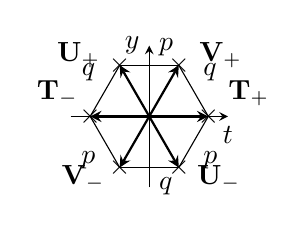
\begin{tikzpicture}[scale=0.5, >=stealth] 
    % Definición de coordenadas (vértices del hexágono)
    \coordinate (O) at (0,0);
    \coordinate (Tp) at (0:1.5);    % T+ (0 grados)
    \coordinate (Vp) at (60:1.5);   % V+ (60 grados)
    \coordinate (Up) at (120:1.5);  % U+ (120 grados)
    \coordinate (Tm) at (180:1.5);  % T- (180 grados)
    \coordinate (Vm) at (240:1.5);  % V- (240 grados)
    \coordinate (Um) at (300:1.5);  % U- (300 grados)

    % Ejes de coordenadas
    \draw[->, thin] (-2,0) -- (2,0) node[below] {$t$};
    \draw[->, thin] (0,-1.8) -- (0,1.8) node[left] {$y$};

    % Lados del hexágono y etiquetas p, q
    % La imagen muestra: 
    % Superior: p, Inferior: q
    % Diagonales superiores: q, Diagonales inferiores: p
    
    \draw (Up) -- node[above right] {$p$} (Vp);           % Superior
    \draw (Vp) -- node[above right] {$q$} (Tp);     % Superior derecha
    \draw (Tp) -- node[below right] {$p$} (Um);     % Inferior derecha
    \draw (Um) -- node[below right] {$q$} (Vm);           % Inferior
    \draw (Vm) -- node[below left] {$p$} (Tm);      % Inferior izquierda
    \draw (Tm) -- node[above left] {$q$} (Up);      % Superior izquierda

    % Vectores (Flechas gruesas desde el origen)
    \draw[->,  thick] (O) -- (Tp) node[pos=0.75, above right] {\;\; $\textbf{T}_+$};
    \draw[->,  thick] (O) -- (Vp) node[pos=0.75, above] {\qquad\quad \;\;$\textbf{V}_+$};
    \draw[->,  thick] (O) -- (Up) node[pos=0.75, above] {$\textbf{U}_{+}$ \qquad \quad \,};
    \draw[->,  thick] (O) -- (Tm) node[pos=0.75, above left] {$\textbf{T}_-$ \; };
    \draw[->,  thick] (O) -- (Vm) node[pos=0.75, below left] {$\textbf{V}_-$\;\,};
    \draw[->,  thick] (O) -- (Um) node[pos=0.75, below right] {\;\;$\textbf{U}_-$};

    % Cruces en los vértices
    \foreach \x in {Tp, Vp, Up, Tm, Vm, Um}
        \node at (\x) {$\times$};

\end{tikzpicture}

\end{minipage}


\section{REPRESENTACIONES IRREDUCIBLES SU(3)}
$\bullet$ \textbf{Diagramas de Peso:} Los estados forman hexágonos o triángulos en el plano $(T_3, Y)$.
\\$\bullet$ \textbf{Etiquetado $(p,q)$:} $p, q$ enteros $\geq 0$. Relacionados con longitud lados polígono en frontera.\\
$\bullet$ \textbf{Dimensión:} $ d(p,q) = \frac{1}{2}(p+1)(q+1)(p+q+2)$

$\bullet$ \textbf{Irreps Importantes:}\\
1. \textbf{Fundamental $\mathbf{3}$:} $(p,q)=(1,0)$.
   Quarks ($u, d, s$):  $u(\frac{1}{2}, \frac{1}{3}), d(-\frac{1}{2}, \frac{1}{3}), s(0, -\frac{2}{3})\quad (\triangle)$\\
2. \textbf{Antifundamental $\bar{\mathbf{3}}$:} $(p,q)=(0,1)$.
   Antiquarks ($\bar{u}, \bar{d}, \bar{s}$). \quad($\bigtriangledown$)\\
3. \textbf{Singlete $\mathbf{1}$:} $(p,q)=(0,0)$.\quad ($\bullet$)\\
4. \textbf{Octete $\mathbf{8}$:} $(p,q)=(1,1)$.
   \hyperlink{Mesones}{Mesones} espín 0, \hyperlink{Bariones}{Bariones} espín 1/2. \hyperlink{Gluones}{Gluones}. Rep. Adjunta.\\
5. \textbf{Decuplete $\mathbf{10}$:} $(p,q)=(3,0)$.
   \hyperlink{Bariones_big}{Bariones} espín 3/2 (Resonancias $\Delta, \Omega^-$).\\
6. \textbf{Sextete $\mathbf{6}$:} $(2,0)$ y $\bar{\mathbf{6}} (0,2)$.\\
$\bullet$ \textbf{Conjugada:} $\textbf{X}\neq\bar{\textbf{X}}$ equivalentemente $(p,q)\neq(q,p)$ (es representación c.c.). Solo: $\textbf{8}=\bar{\textbf{8}}$.\\
$\bullet$ \hyperlink{young}{\textbf{Productos Tensoriales de Irreps}} (ejemplos): $\textbf{8} \otimes {\textbf{8}} = \textbf{1} \oplus {\textbf{8}} \oplus \textbf{8} \oplus \textbf{10}\oplus \overline{\textbf{10}} \oplus {\textbf{27}}$\\
$\textbf{3} \otimes \bar{\textbf{3}} =\textbf{8}\oplus \textbf{1}$\quad$\textbf{3} \otimes {\textbf{3}} = \textbf{6} \oplus \bar{\textbf{3}}$\quad$\textbf{3} \otimes {\textbf{6}} = \textbf{8} \oplus {\textbf{10}}$\quad$\textbf{3} \otimes {\textbf{3}} \otimes \textbf{3} = \textbf{1} \oplus {\textbf{8}} \oplus \textbf{8} \oplus \textbf{10}$


\section{PROPIEDADES ALGEBRAICAS}
$\bullet$ Los productos directos cumplen propiedades distributivas, asociativas y conmutativas respecto a la suma directa.\\
$\bullet$ \textbf{Isospin Agrandado:} $SU(2) \subset SU(3)$. Las interacciones fuertes conservan $SU(3)$ (aproximadamente) y $SU(2)$ (con mayor precisión).


\section{CLASIFICACIÓN DE HADRONES -- SU(3)$_F$ (F$\equiv$ flavour)}
-- Solo podemos observar partículas libres (estados ligados) neutras de color (singletes) --
\textbf{Mesones ($q\bar{q}$)}:
Descomposición en $SU(3)_F$: $ \mathbf{3} \otimes \mathbf{\bar{3}} = \mathbf{1} \oplus \mathbf{8} $\\
\textbf{Bariones ($qqq$)}:
Descomposición en $SU(3)_F$:
$ \mathbf{3} \otimes \mathbf{3} \otimes \mathbf{3} = \mathbf{1} \oplus \mathbf{8} \oplus \mathbf{8} \oplus \mathbf{10} $\\
$\bullet$ SU(2)$_I$ (Isospín): Muy buena simetría ($m_u \approx m_d$).\\
$\bullet$ SU(3)$_F$ (Sabor): Simetría rota ($m_s > m_{u,d}$) $\Rightarrow \Delta m$ dentro de los multipletes.\\
$\bullet$ $\nexists$ SU(4) o superiores como simetrías aproximadas debido a la gran masa de $c, b, t$.



\section{FUNCIONES DE ONDA (MODELO ESTÁTICO)}
Función de onda total de un hadrón:
$\Psi_{\text{tot}} = \Psi_{\text{espacio}} \times \Psi_{\text{sabor}} \times \Psi_{\text{spin}} \times \Psi_{\text{color}} $\\
$\Psi_{\text{tot}}$ \textbf{totalmente antisimétrica} (fermiones), \textbf{totalmente simétrica} (bosones).

\textbf{Construcción del Protón ($p^\uparrow$)}:\\
-- Paridad $\Psi_{\text{espacio}}$: $(-1)^L$. Estado fundamental ($L=0$) $\implies$ 
simétrica.\\
Combinación Flavor-Spin debe ser simétrica (para compensar antisimetría de color).\\
Base de Flavour ($uud$):\\
$\bullet$ Simétrica ($1\leftrightarrow 2$): $\phi_S = \frac{1}{\sqrt{6}}[(ud+du)u - 2uud]$.\\
$\bullet$ Antisimétrica ($1\leftrightarrow 2$): $\phi_A = \frac{1}{\sqrt{2}}(ud-du)u$.\\
Base de Spin ($\uparrow\uparrow\downarrow$):\\
$\bullet$ Simétrica ($1\leftrightarrow 2$): $\chi_S = \frac{1}{\sqrt{6}} [\uparrow\downarrow\uparrow + \downarrow\uparrow\uparrow -2 \uparrow\uparrow\downarrow]$ (Espín 1).\\
$\bullet$ Antisimét ($1\leftrightarrow 2$): $\chi_A = \frac{1}{\sqrt{2}} [\uparrow\downarrow\uparrow-\downarrow\uparrow\uparrow]$ (Espín 0).\\
-- \text{Función Flavour-Spin}: $ \Psi_{F-S}(p^\uparrow) = \frac{1}{\sqrt{2}} (\phi_S \chi_S + \phi_A \chi_A) $ = 
$$= | p \uparrow\rangle   = \frac{1}{\sqrt{18}} [2|u\!\uparrow u\!\uparrow d\!\downarrow\rangle - |u\!\uparrow u\!\downarrow \!d\uparrow\rangle - |u\!\downarrow u\!\uparrow d\!\uparrow\rangle + \text{perms} ] $$
perms: permutaciones \underline{cíclicas} de los pares (quarks-espín)

\section{MOMENTOS MAGNÉTICOS}
Operador: $\vec{\mu} = \sum_i \mu_i \vec{\sigma}_i$.
Donde $\mu_q = Q_q (\frac{e}{2m_q})$.
Valor esperado $\langle p\uparrow | \mu_z | p\uparrow \rangle$:
$$ \mu_p = \frac{1}{3}(4\mu_u - \mu_d) \qquad  \mu_n = \frac{1}{3}(4\mu_d - \mu_u) $$




\section{COLOR SU(3)$_c$}
\textbf{Carga de Color}: $R= \textbf{q}_1,\,G=\textbf{q}_2, \, B = \textbf{q}_3$ (Fundamental $\mathbf{3}$ de $SU(3)_c$).\\
\textbf{Confinamiento}:
Los hadrones observados son \textbf{Singletes de Color} ($\mathbf{1}$).\\
$\Psi_{\text{color}}$ debe ser totalmente antisimétrica e invariante bajo rotaciones en el espacio de color.


\textbf{Singlete Bariónico ($qqq$)}:
$ \mathbf{1} \in \mathbf{3} \otimes \mathbf{3} \otimes \mathbf{3} $
$$ \Psi_{\text{color}} = \frac{1}{\sqrt{6}} \epsilon_{ijk} |q_i q_j q_k\rangle = \frac{1}{\sqrt{6}}(RGB - RBG + BRG - BGR + GBR - GRB) $$

\textbf{Singlete Mesónico ($q\bar{q}$)}:
$ \mathbf{1} \in \mathbf{3} \otimes \mathbf{\bar{3}} $
$$ \Psi_{\text{color}} \!=\! \frac{1}{\sqrt{3}} (R\bar{R} + G\bar{G} + B\bar{B}) \quad \bar{R}= \frac{1}{\sqrt{2}} (GB-BG)\quad \bar{G} =  \frac{1}{\sqrt{2}} (BR-RB)\quad  \bar{B} = \frac{1}{\sqrt{2}} (RG-GR)$$


\section{MODELO DE PARTONES (FEYNMAN 1969)}
\textbf{Composición Hadrones:}\\
$\bullet$ \textbf{Quarks de valencia ($q_v$):} Definen n$^\text{os}$ cuánticos. e.g.: $p$ ($u_v u_v d_v$), $n$ ($d_v d_v u_v$).\\
$\bullet$ \textbf{Partones del mar (Sea Partons):} Pares $q\bar{q}$ (prob< no nula de excitación) y gluones ($g$). Participan en reparto energético, no en números cuánticos globales. \\

\textbf{Cinemática (Infinite Momentum Frame):}\\
$\bullet$ Protón con momento $P$ y energía $E$. Partón $i$ lleva fracción $x$ del momento. \\
$\bullet$ \textbf{Variable de Bjorken:} $x = p_{\text{parton}}/P_{\text{proton}}$, con $0 \le x \le 1$. \\
$\bullet$ Momentos: $p_i^\mu \approx x P^\mu$. Transverso ($\perp$) $P_T \approx 0$, Longitudinal ($\parallel$) $P_L \neq0$ (respecto haz). \\
$\bullet$ Masa hadrón y partones se desprecian a altas energías ($s \gg M^2$).

\section{FUNCIONES DE DISTRIBUCIÓN DE PARTONES (PDFs)}
\textbf{PDF ($f_i(x)$):}
Probabilidad de hallar partón tipo $i$ con fracción de momento $x$ en el hadrón.\\
$\bullet$ \textbf{Regla de suma (Momentum Sum Rule):} Conservación del momento total del protón.
$$ \sum_{i} \int_0^1 x f_i(x) dx = 1 $$
La suma $i$ incluye valencia, sea y gluones. Experimentos: gluones $\sim 50\%$ del momento.

\textbf{Tipos y Nomenclatura:}\\
$\bullet$ Valencia: $u_v, d_v$. Sea: $u_s, d_s, s_s, \dots$ y antiquarks $\bar{u}, \bar{d}, \bar{s}$. \\
$\bullet$ Simetría del mar: $q_s(x) = \bar{q}_s(x)$. \\
$\bullet$ PDFs totales: $u(x) = u_v(x) + u_s(x)$, $\bar{u}(x) = \bar{u}_s(x)$. \\
$\bullet$ Protón tiene $2u$ y $1d$: $\int_0^1 (u(x)-\bar{u}(x))dx = 2$, $\int_0^1 (d(x)-\bar{d}(x))dx = 1$.

\textbf{Comportamiento ``Naive":}\\
$\bullet$ \textbf{Valencia:} Domina en $x \sim 1/3$. \\
$\bullet$ \textbf{Sea/Gluones:} Dominan a bajo $x$ ($x \to 0$). Divergencia infrarroja regularizada.

\section{TEOREMA DE FACTORIZACIÓN}
Separación del proceso hadrónico en:\\
1. \textbf{Soft Physics:} PDFs (No perturbativo, universal).\\
2. \textbf{Hard Physics:} Sección eficaz partónica $\hat{\sigma}$ (Perturbativo, calculable).

\textbf{Fórmula General (Colisión $P_1 + P_2$):}
$$ \sigma_{\text{tot}}(s) = \sum_{i,j} \int_0^1 dx_1 \int_0^1 dx_2 f_i(x_1) f_j(x_2) \hat{\sigma}_{ij}(\hat{s}) $$
$\bullet$ $x_{1,2}$: Fracción momento partones 1 y 2. \\
$\bullet$ $s = (P_1+P_2)^2 \approx 2P_1 P_2$. \\
$\bullet$ $\hat{s} = (x_1 P_1 + x_2 P_2)^2 \approx x_1 x_2 s$. \\
$\bullet$ $\hat{\sigma}_{ij}$: Sección eficaz subproceso elemental $i+j \to \text{final}$.



\section{PROCESOS DE COLISIÓN ESPECÍFICOS}
\textbf{1. Electrón-Protón ($ep \to e^- X$, DIS):}
Sonda: Fotón virtual $\gamma^*$ (o $Z$) con $Q^2 = -q^2$.
$$ \sigma(ep \to eX) = \sum_i \int_0^1 dx f_i(x) \hat{\sigma}(eq_i \to eq_i) $$
$\bullet$ Diagrama: Scattering $e^-$ sobre quark libre $q_i$. \\
$\bullet$ Estado final: $e^-$ saliente + Jet hadrónico (quark) + Remanente protón (dirección haz).

\textbf{2. Protón-Antiprotón ($p\bar{p} \to \ell^+\ell^- X$, Drell-Yan):}
Aniquilación $q_i \bar{q}_i \to \gamma^*/Z \to \ell^+ \ell^-$.
$$ \sigma = \sum_{i} \int dx_1 dx_2 [f_i(x_1) f_{\bar{i}}(x_2) + f_{\bar{i}}(x_1) f_i(x_2)] \hat{\sigma}(q\bar{q} \to \ell\ell) $$
$\bullet$ Requiere un quark de valencia y un antiquark (valencia en $\bar{p}$ o sea en $p$).

\textbf{3. Protón-Protón ($pp \to W^\pm X$):}
Producción bosón $W$ vía interacción débil.
$$ \sigma = \sum_{i,j} \int dx_1 dx_2 f_i(x_1) f_j(x_2) V_{CKM}^2 \hat{\sigma}(q_i \bar{q}_j \to W) $$
$\bullet$ Ejemplo $u \bar{d} \to W^+$. Antiquark debe provenir del mar (sea) en colisiones $pp$.

\section{FUNCIONES DE ESTRUCTURA Y $Q^2$}
\textbf{Función $F_2(x, Q^2)$:}
Relaciona sección eficaz medida con contenido partónico.
$$ F_2(x, Q^2) = \sum_i e_i^2 x f_i(x, Q^2) $$
$\bullet$ $e_i$: Carga eléctrica quark ($u=2/3, d=-1/3$). \\
    $\bullet$ Gluones no contribuyen directamente a $F_2$ en orden más bajo (LO), solo q/$\bar{\text{q}}$ cargados.

\textbf{Scaling de Bjorken:}\\
$\bullet$ Predicción Partones (Naive): $F_2(x, Q^2) \to F_2(x)$. Indep de $Q^2$ si partones puntuales.\\
$\bullet$ \textbf{Violación del Scaling:} Experimentalmente $F_2$ depende de $Q^2$.\\
- $x$ bajos: $F_2$ crece con $Q^2$ (aumenta densidad partones sea/gluones al aumentar resolución).\\
- $x$ altos: $F_2$ decrece con $Q^2$ (quarks valencia radian gluones y pierden momento).

\section{EVOLUCIÓN QCD (DGLAP)}
El modelo de partones estático no predice dependencia en $Q^2$. QCD introduce evolución vía emisión de gluones (splitting).\\
$\bullet$ Escala $Q^2$: Resolución espacial probe $\sim 1/\sqrt{Q^2}$.\\
$\bullet$ \textbf{Ecuaciones DGLAP:} Describen variación de PDFs con $\ln Q^2$.\\

\textbf{Ejemplo (Evolución del Gluón):}
$$ \frac{d g(x,Q^2)}{d \ln Q^2} = \frac{\alpha_s(Q^2)}{2\pi} \int_x^1 \frac{dy}{y} \left[ \sum_q P_{gq}\left(\frac{x}{y}\right) q(y,Q^2) + P_{gg}\left(\frac{x}{y}\right) g(y,Q^2) \right] $$
$\bullet$ $\alpha_s$: Constante acoplamiento fuerte. \\
$\bullet$ $P_{ba}(z)$: Funciones de splitting. Probabilidad proceso $a \to b$ con fracción $z$.\\
- $P_{qq}$: Quark radia gluón (queda quark).\\
- $P_{gq}$: Quark radia gluón (queda gluón).\\
- $P_{gg}$: Gluón se divide en gluones ($g \to gg$).\\
- $P_{qg}$: Gluón crea par $q\bar{q}$.\\


